
\documentclass[12pt]{article}
\usepackage{geometry}
\linespread{2}
\geometry{a4paper,scale=0.8}
\usepackage{mathrsfs}
\usepackage[UTF8]{ctex}
\usepackage{amsmath}
\usepackage{algorithm} 
\usepackage{algorithmic}
\usepackage{amsfonts}
\usepackage{multirow}
\usepackage{booktabs}
\usepackage{graphicx} 
\usepackage{subfigure}
\usepackage{float}
\usepackage{bm}
\usepackage{latexsym}
\usepackage{tikz}


\begin{document}
	\section{优化目标}
	考虑如下group LASS问题:
	$$
	\min _{x \in \mathbb{R}^{n \times l}} \frac{1}{2}\|A x-b\|_F^2+\mu\|x\|_{1,2}
	$$
	其中$A \in \mathbb{R}^{m \times n}, b \in \mathbb{R}^{m \times l}$,给定 $\mu>0$ ,$\|x\|_{1,2}$由如下给出:
	$$
	\|x\|_{1,2}=\sum_{i=1}^n\|x(i, 1: l)\|_2 .
	$$
	\section{cvx求解}
	利用python中的cvxpy包,如下为调用mosek和gurobi求解器得到的解,其中解为$n\times l$矩阵,按列将解画在图上:
\begin{figure}[H]
\centering
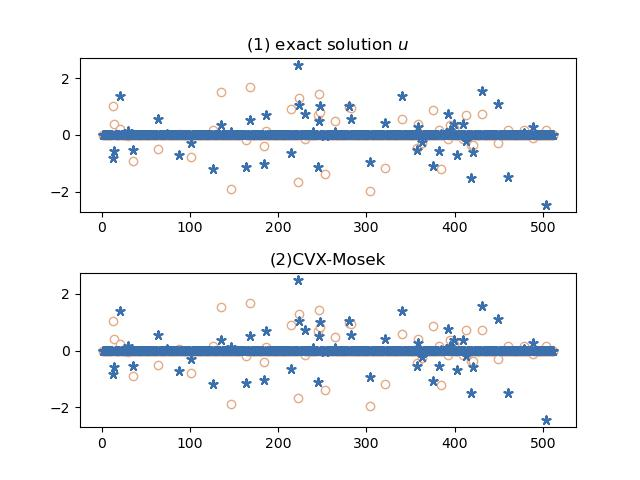
\includegraphics[width=\textwidth]{figs/CVX-Mosek.jpg}
\caption{CVX-Mosek解与精确解$u$对比}
\end{figure}

\begin{figure}[H]
	\centering
	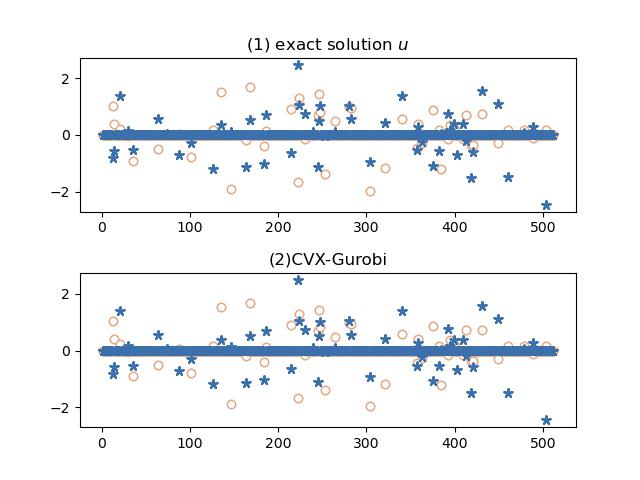
\includegraphics[width=\textwidth]{figs/CVX-Gurobi.jpg}
	\caption{CVX-Gurobi得到的解与精确解$u$对比}
\end{figure}
	
	\section{mosek求解器和gurobi求解器}
	
	在调用mosek和gurobi前,现将原问题转化为如下等价的二次规划和二次锥约束问题:
	\begin{equation*}
		\begin{aligned}
			&\min \limits_{x,t} \frac{1}{2}\|A x-b\|_F^2 + \mu \textbf{1} t\\
			&\mathrm{s.t.} \Vert x(i,1:l) \Vert \leq t_i, i = 1,2,\cdots, n
		\end{aligned}
	\end{equation*}    
其中向量$  \textbf{1}  \in \mathcal{R}^{n}$,下面展示了具体结果:                          
		\begin{figure}[H]
		\centering
		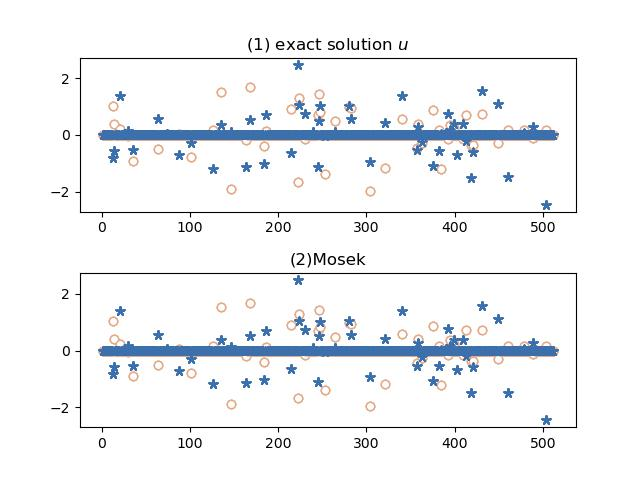
\includegraphics[width=\textwidth]{figs/Mosek.jpg}
		\caption{Mosek得到的解与精确解$u$对比}
	\end{figure}
	\begin{figure}[H]
		\centering
		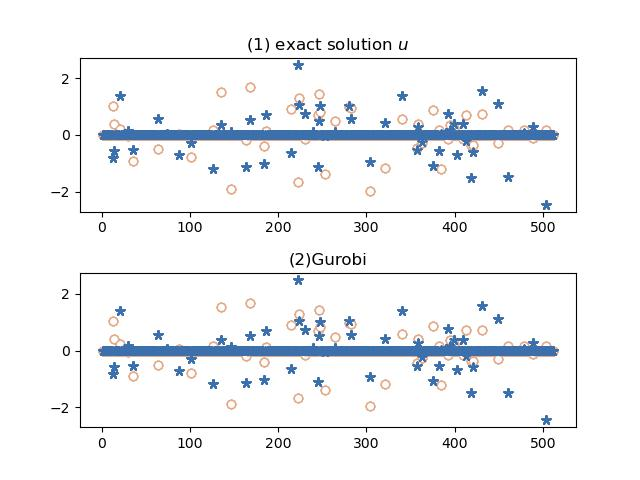
\includegraphics[width=\textwidth]{figs/Gurobi.jpg}
		\caption{Gurobi得到的解与精确解$u$对比}
	\end{figure}


	\section{次梯度法}

	对于函数 $f(x)=\frac{1}{2}\|A x-b\|_F^2+\mu\|x\|_{1,2}$, 它的次梯度可以表示如下
	$$
	\partial f(x)=A^T A x-A^T b+\mu  \partial \|x\|_{1,2}
	$$
	其中\begin{equation*}
		\partial \|x\|_{1,2} = \left[\begin{array}{c}
		 \partial x(1,1:l)\\
			\partial x(2,1:l)\\
			\vdots\\
		\partial x(n,1:l)\\
		\end{array} \right]
	\end{equation*}
\begin{equation*}
	\partial x(i,1:l) = 	\left\{
	\begin{array}{ll}
		\frac{x(i,1:l)}{\Vert x(i,1:l) \Vert_2}, &   x(i,1:l)\neq \mathbf{0}\\
		\left\{w \mid\Vert w \Vert_2  \leq 1 \right\}, & x(i,1:l) = \mathbf{0}
	\end{array}
	\right.
\end{equation*}

利用辅助函数确定当前步步长, 然后进行一步次梯度法迭代 $x^{k+1}=x^k-\alpha_k g\left(x^k\right)$ 。其中 $g\left(x^k\right) \in \partial f\left(x^k\right)$ 。
	题目中 $\mu$ 的值过小, 直接求解收敛速度过慢, 所以先从较大的 $\mu$ 开始,采用连续化策略,直到$mu$衰减到题目中要求的值。
	\begin{figure}[H]
	\centering
	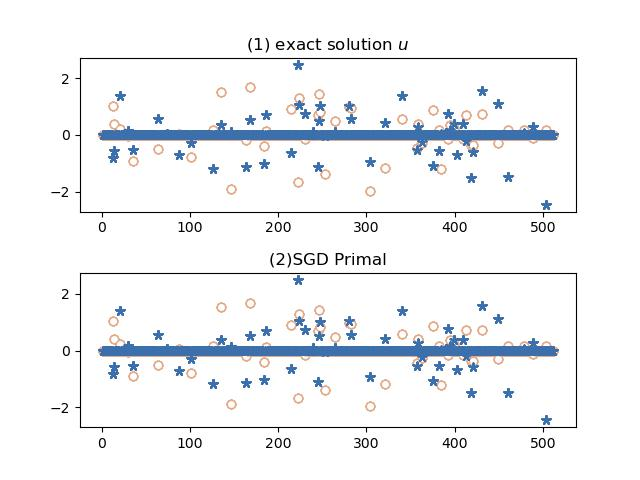
\includegraphics[width=\textwidth]{figs/SGD Primal.jpg}
	\caption{SGD得到的解与精确解$u$对比}
\end{figure}
	
	

	
	
	\section{近似点梯度法}
	
优化问题可以看作$f(x) = \phi(x) + h(x)$,其中$ \phi(x) = \frac{1}{2}\|A x-b\|_F^2, \ h(x) =\mu\|x\|_{1,2}$.
题目中 $\mu$ 的值过小, 直接求解收敛速度过慢, 采用连续化策略,连续化策略从较大的正则化参数 $\mu_t$ 逐渐减小到 $\mu$ (即 $\mu_1 \geq \cdots \geq \mu_{t-1} \geq \mu_t \geq \cdots \geq \mu$ ), 并求解相应的 LASSO 问题:

  事实上,近似点梯度法的迭代格式根据定义可以写为 

 $$ \begin{array}{ll} x^{k+1}&\hspace{-0.5em}=\displaystyle\arg\min_u
	 \left(  \mu_k \|u\|_{1,2}+\frac{1}{2 \alpha_k}\|u-x^k+ \alpha_k\nabla \phi(x^k)\|_2^2 \right)  \\
	 &\hspace{-0.5em}=\displaystyle\arg\min_u \left(   \mu_k  \|u\|_{1,2}+\phi(x^k)
	 +\nabla \phi(x^k)^\top (u-x^k)+\frac{1}{2 \alpha_k}\|u-x^k\|^2_2 \right).
	 \end{array} $$

%%
 检验是否满足非精确线搜索条件,针对 $f(x)$ 考虑线搜索准则,即为 $f(x^{k+1}(t))\le C_k - \frac{1}{2}\rho t
 \| x^{k+1}(t)-x^k\|^2$,其中 $x^{k+1}(t) = \mathrm{prox}_{\mu_k \Vert \cdot \Vert_{1,2}}(x^k -\alpha_k \nabla \phi(x^k))$。 

 |nls| 记录线搜索循环的迭代次数,
 直到满足条件或进行10次步长衰减后退出线搜索循环,得到更新的 $x^{k+1}$。 $C_k$ 为 (Zhang \&
 Hager) 线搜索准则中的量。如果不满足线搜索条件,对当前步长进行衰减,当前线搜索次数加一。
 线搜索结束,得到更新的 $x, g$。计算梯度范数和原始目标函数值。 fvec 记录每一步对应的原 LASSO 问题的目标函数值。并进行内层循环的收敛判断: 若当前梯度小于阈值或者目标函数变化小于阈值,内层迭代终止。
 
 计算 BB 步长作为下一步迭代的初始步长。令 $s^k=x^{k+1}-x^k, y^k=g^{k+1}-g^k$, 这里在偶数与奇数步分别对应 $\frac{\left(s^k\right)^{\prime} s^k}{\left(s^k\right)^{\top} y^k}$ 和 $\frac{\left(s^k\right)^{\top} y^k}{\left(y^k\right)^{\top} y^k}$ 两个 BB 步长。
 
 得到如下结果:
 
 
 	\begin{figure}[H]
 	\centering
 	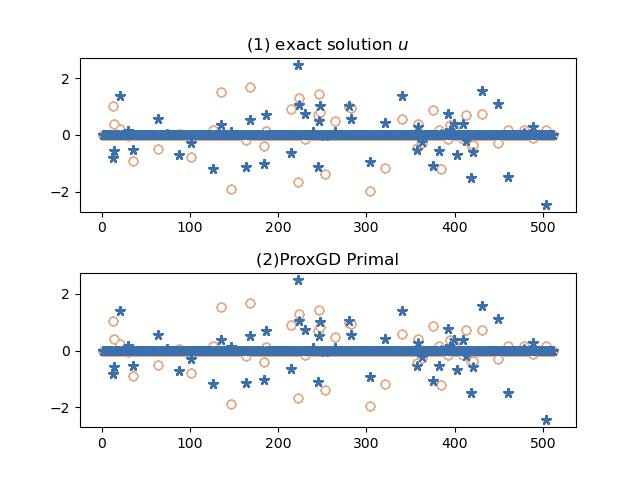
\includegraphics[width=\textwidth]{figs/ProxGD Primal.jpg}
 	\caption{ProxGD得到的解与精确解$u$对比}
 \end{figure}
 
 
 \section{FProxGD算法}
 利用 Nesterov 加速的近似点梯度法进行优化。
 该算法被外层连续化策略调用,在连续化策略下完成某一固定正则化系数的内层迭代优化。
 在每一步迭代时, 算法首先在之前两步迭代点的基础上进行一步更新 $y^k=x^{k-1}+\frac{k-2}{k+1}\left(x^{k-1}-x^{k-2}\right)$, 然后再在 $y^k$ 处进行一步近似点梯度法, $x^k=\operatorname{prox}_{\mu_k \|\cdot\|_{1,2} }\left(y^k-t_k A^{\top}\left(A y^k-b\right)\right.$ 。
 
 	\begin{figure}[H]
 	\centering
 	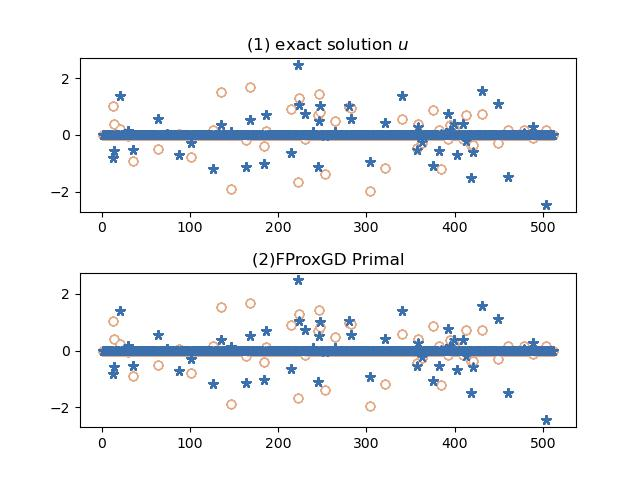
\includegraphics[width=\textwidth]{figs/FProxGD Primal.jpg}
 	\caption{FProxGD得到的解与精确解$u$对比}
 \end{figure}
 
 
 \section{对偶问题的ALM算法}
 原问题等价于
 \begin{equation*}
 	\begin{aligned}
 		\min \limits_{x,z}&  \frac{1}{2}\|z-b\|_F^2+\mu\|x\|_{1,2}\\
 		\text{s.t. }& Ax-z=0
 	\end{aligned}
 \end{equation*}

 构造拉格朗日函数$L(x,z,y) = \frac{1}{2}\|y-b\|_F^2-\langle z, y\rangle+\mu\|x\|_{1,2}+\left\langle A^T y, x\right\rangle $
 通过最小化$x$ 和 $z$,我们有:
 $$
 \begin{aligned}
 	g(y) & =\inf _{x, z} L(x, z, y)=\inf _{x, z}  \frac{1}{2}\|y-b\|_F^2-\langle z, y\rangle+\mu\|x\|_{1,2}+\left\langle A^T y, x\right\rangle \\
 	& =-\frac{1}{2}\|y\|_F^2-\langle b, y\rangle+I\left[\left\|A^T y\right\|_{\infty, 2}^* \leq \mu\right]
 \end{aligned}
 $$
 因此原问题的对偶问题为:
 $$
 \begin{array}{cl}
 	\min _y & \frac{1}{2}\|y\|_F^2+\langle b, y\rangle \\
 	\text { s.t } & \left\|A^T y\right\|_{\infty, 2} \leq \mu .
 \end{array}
 $$
其中矩阵的$(\infty, 2)$范数定义为$\|A\|_{\infty, 2}=\max _i\|A(i, 1: l)\|_2$,为了避免复杂的符号 $\left\|A^T z\right\|_{\infty, 2}$,引入等式约束,使得ALM 算法更加的平滑。
 $$
 \begin{array}{ll}
 	\min _y & \frac{1}{2}\|y\|_F^2+\langle b, y\rangle \\
 	\text { s.t } & \|s\|_{\infty, 2} \leq \mu, s=A^T y
 \end{array}
 $$
 它的增广拉格朗日函数为:
 $$
 L^d(y, s, \lambda, \mu)=\frac{1}{2}\|y\|_F^2+\langle b, y\rangle+\left\langle\lambda, A^T y-s\right\rangle+\frac{\sigma}{2}\left\|A^T y-s\right\|_F^2
 $$
 以及约束 $\|s\|_{\infty, 2} \leq \mu$。因此对偶问题的增广拉格朗日函数法对于每个固定的$\lambda$解决如下子问题:
 $$
 \begin{array}{ll}
 	\min _{y,s} & \frac{1}{2}\|y\|_F^2+\langle b, y\rangle+\left\langle\lambda, A^T y -s\right\rangle+\frac{\sigma}{2}\left\|A^T y -s\right\|_F^2 \\
 	\text { s.t } & \|s\|_{\infty, 2} \leq \mu
 \end{array}
 $$
 \subsection{迭代格式}
 上述对偶问题的增广拉格朗日函数法的迭代格式为
 \begin{equation*}
 \left\{	\begin{array}{l}
 	(y^{k+1},s^{k+1}) =\mathop{\arg\min}\limits_{y,\|s\|_{\infty, 2} \leq \mu}  L^d(y, s, \lambda^k, \mu)=\mathop{\arg\min}\limits_{y,\|s\|_{\infty, 2} \leq \mu} \left\{\frac{1}{2}\|y\|_F^2+\langle b, y\rangle+\frac{\sigma_k}{2}\left\|A^T y -s+\frac{\lambda}{\sigma_k}\right\|_F^2 \right\}\\
 	\lambda^{k+1} = \lambda^{k}+\sigma_k(A^{\top}y^{k+1}-s^{k+1})\\
 	\sigma_{k+1} = \min \left\{\rho \sigma_k,\bar{\sigma}\right\}
 \end{array}\right.
 \end{equation*}
其中$\rho >1$和$\bar{\sigma}< +\infty$为算法参数,由于$(y^{k+1},s^{k+1})$的显式表达式是未知的,我们需要利用迭代算法来进行求解。

首先关于$y$的极小化问题为:
\begin{equation*}
	\begin{aligned}
		\min \frac{1}{2}\|y\|_F^2+\langle b, y\rangle+\left\langle\lambda, A^T y -s\right\rangle+\frac{\sigma}{2}\left\|A^T y -s\right\|_F^2
	\end{aligned}
\end{equation*}
进一步化简可知:
$$
y = \mathop{\arg\min}_y \operatorname{tr}\left(\frac{1}{2}\|y\|_F^2+\frac{1}{2}y^{\top} (\sigma_k A A^{\top}) y + (b^{\top}+\lambda^{\top} A^{\top}-\sigma_k s^{\top}A^{\top})y \right)
$$
 设$h(y) = \frac{1}{2}^{\top} (\sigma_k A A^{\top}) y + (b^{\top}+\lambda^{\top} A^{\top}-\sigma_k s^{\top}A^{\top})y $,那么$y = \operatorname{prox}_h(0) = \mathop{\arg\min}\limits_{u}\operatorname{tr}\left\{ h(u)+\frac{1}{2}\|y\|_F^2\right\}$,有二次函数的近似算法可知$y = \left(I + \sigma_k A A^{\top}\right)^{-1} (\sigma_k As-A \lambda-b)$
 
 关于$s$的极小化问题为:
 \begin{equation*}
 	\begin{aligned}
 		& \min_s \frac{\sigma_k}{2}\left\|A^T y -s+\frac{\lambda}{\sigma_k}\right\|_F^2\\
 		&\text{s.t.} \|s\|_{\infty, 2} \leq \mu
 	\end{aligned}
 \end{equation*}
通过简单的推导可知:
$$
s = \mathcal{P}_{\|s\|_{\infty, 2} \leq \mu}\left(A^T y +\frac{\lambda}{\sigma_k}\right)
$$
 
 \subsection{优化结果}
  	\begin{figure}[H]
 	\centering
 	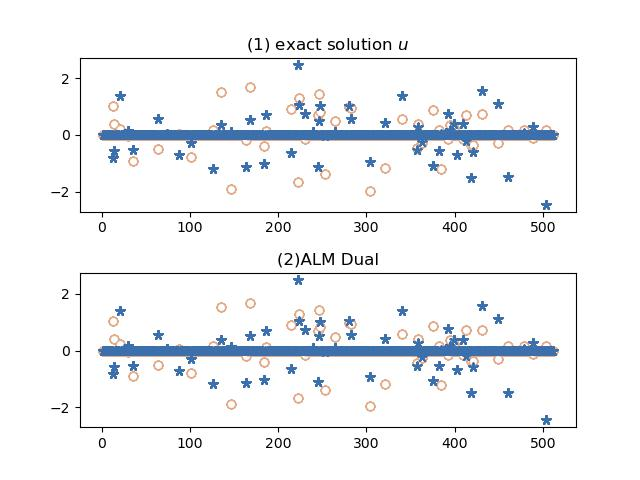
\includegraphics[width=\textwidth]{figs/ALM Dual.jpg}
 	\caption{ALM Dual得到的解与精确解$u$对比}
 \end{figure}
 
 
 
  \section{对偶问题的ADMM算法}
    	\begin{figure}[H]
  	\centering
  	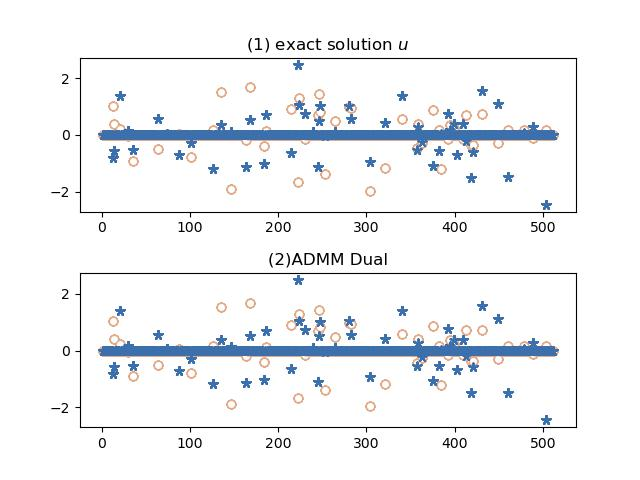
\includegraphics[width=\textwidth]{figs/ADMM Dual.jpg}
  	\caption{ADMM Dual得到的解与精确解$u$对比}
  \end{figure}
  
  
    \section{原问题的ADMM算法}
    	\begin{figure}[H]
    	\centering
    	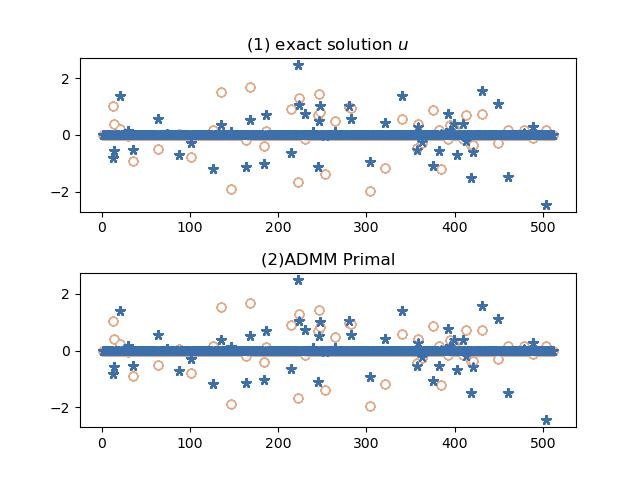
\includegraphics[width=\textwidth]{figs/ADMM Primal.jpg}
    	\caption{ADMM Primal得到的解与精确解$u$对比}
    \end{figure}
    
    \section{总结}
    \begin{table}[H]
    	\centering
    	\caption{比较不同算法的效率}
    	\resizebox{\textwidth}{3.5cm}{
    \begin{tabular}{r|ccccccc}
    \toprule
    	Solver & Time(s) & Iter &  Fval &  Sparisity & Errfun-Exact &  Errfun-CVX-Mosek & Errfun-CVX-Gurobi \\
    \midrule
    CVX-Mosek& 0.46&  9 &5.42980E-01 &0.294& 4.21E-05& 0.00E+00& 1.47E-06\\
    CVX-Gurobi &3.86&16&5.42980E-01&0.328&4.33E-05&1.47E-06& 0.00E+00\\
    Mosek& 0.25&   10&5.42980E-01&0.291& 4.19E-05& 2.94E-07&1.72E-06\\
    Gurobi&4.20& 14 & 5.42986E-01&0.750&4.72E-05&6.43E-06&5.14E-06\\
    SGD Primal &19.12&  100&5.42983E-01&0.578&5.79E-05&1.90E-05& 1.79E-05\\
    ProxGD Primal&22.34& 13 &5.42980E-01& 0.291&4.19E-05&3.11E-07& 1.73E-06\\
    FProxGD Primal&4.99&  6& 5.42980E-01&0.291& 4.19E-05&3.19E-07& 1.74E-06\\
    ALM Dual & 1.54&283&5.42997E-01&0.248&7.59E-05&4.33E-05&4.26E-05\\
    ADMM Dual& 0.69&  76& 5.42998E-01& 0.248&8.07E-05& 4.67E-05& 4.59E-05\\
    ADMM Primal & 9.52 & 2392 & 5.42980E-01& 0.291& 4.19E-05 & 3.21E-07& 1.71E-06\\
    \bottomrule
    \end{tabular}	}
    \end{table}
 
\end{document}
